\documentclass{beamer}
%\documentclass[handout]{beamer}

% This file is a solution template for:
% PHYS3202 Lectures
\mode<presentation>
{
  \usetheme{Madrid}
  \setbeamercovered{invisible}
\setbeamertemplate{footline}[frame number]{}
\setbeamertemplate{navigation symbols}{}
\setbeamertemplate{footline}{}
}
\usepackage[english]{babel}
\usepackage[latin1]{inputenc}
%\usepackage{times}
\usepackage[T1]{fontenc}

\renewcommand\familydefault{\sfdefault}

\usefonttheme[onlymath]{serif}


\usepackage[cm]{sfmath}

\newcommand{\td}[1]{\frac{D #1}{D t}}
\newcommand{\nd}[2]{\frac{d #1}{d #2}}
\newcommand{\ns}[2]{\frac{d^2 #1}{d #2^2}}
\newcommand{\sd}[2]{\frac{D #1}{D #2}}
\newcommand{\pd}[2]{\frac{\partial #1}{\partial #2}}
\newcommand{\ps}[2]{\frac{\partial^2 #1}{{\partial #2}^2}}
\newcommand{\pt}[2]{\frac{\partial^3 #1}{{\partial #2}^3}}
\newcommand{\pst}[3]{\frac{\partial^2 #1}{\partial #2 \partial #3}}
\newcommand{\ptt}[3]{\frac{\partial^3 #1}{{\partial #2}^2 \partial #3}}
\newcommand{\vc}[1]{\mathbf{#1}}
\newcommand{\mtx}[1]{\vc{\mathsf{#1}}}

%\sffamily

\title[Geopotential]{Geopotential}
%\begin{columns}
%  \column{0.5\textwidth}

\author{$\quad\quad\quad\quad\quad\quad\quad\quad\quad\quad\quad\quad\quad\quad$Kial~Stewart}


\institute{
  $\quad\quad\quad\quad\quad\quad\quad\quad\quad\quad\quad\quad\quad\quad\quad\quad\quad\quad$Research School of Earth Sciences\\
  $\quad\quad\quad\quad\quad\quad\quad\quad\quad\quad\quad\quad\quad\quad\quad\quad\quad\quad$e: kial.stewart@anu.edu.au\\
  }

\date{$\quad\quad\quad\quad\quad\quad\quad\quad\quad\quad\quad\quad\quad\quad$PHYS 3202}
%  \column{0.5\textwidth}
  
%  \end{columns}
%%%%%%%%%%%%%%%%%%%%%%%%%%%%%%%

\begin{document}

\begin{frame}
  \titlepage
\end{frame} 

%%%%%%%%%%%%%%%%%%%%%%%%%%%%%%%
%
%\frame{
%\frametitle{Fluid Flow on a Rotating Planet}
%
%Topics:
%\begin{itemize}
%
%\item {Transforming into a Rotating Frame of Reference}
%
%\item {Geopotential Surfaces}
%
%\item {Coriolis Force}
%
%\item {Momentum Equation on a Rotating Planet}
%
%\end{itemize}
%}
%%%%%%%%%%%%%%%%%%%%%%%%%%%%%%%
%
%\frame{
%  \frametitle{Flow in an inertial reference frame}
%  \begin{itemize}
%   \item Continuum fluid motion forced by pressure gradients and gravity:\\
%
%\pause
%   - Continuity equation (incompressible fluid)
%   \[\nabla \cdot \vc{u} = 0\]
%\pause
%   - Navier-Stokes momentum equation
%   \[\sd{\vc{u}}{t} =  \vc{g} - \frac{\nabla p}{\rho} + \nu \nabla^2 \vc{u}\]
%\pause
%   \item For inviscid flow, the horizontal and vertical momentum equations reduce to Euler's equations
%    \[  \sd{u}{t}  = - \frac{1}{\rho}\pd{p}{x} ,  \hskip0.5cm	\sd{v}{t}  = - \frac{1}{\rho}\pd{p}{y}\]
%\pause
%    \[  \sd{w}{t}  = - g - \frac{1}{\rho}\pd{p}{z}\]
%\end{itemize}
%
%\pause
%
% \begin{alertblock}{\textbf{Inertial} reference frame}
% \begin{itemize}
% \item{implies \textbf{flow timescale} $<<$ \textbf{planetary rotation timescale}}
%\end{itemize}
%\end{alertblock}
%}
%
%
%%%%%%%%%%%%%%%%%%%%%%%%%%%%%%%%
%
%\frame{
%  \frametitle{Flow on a Rotating Planet}
%  \begin{columns}
%  \column{0.5\textwidth}
%%   \includegraphics[width=1.0\hsize]{jupiter__1__speedyspacebike.jpg}
%
%  \column{0.5\textwidth}
%  \vskip5cm
%
%%\pause
%%  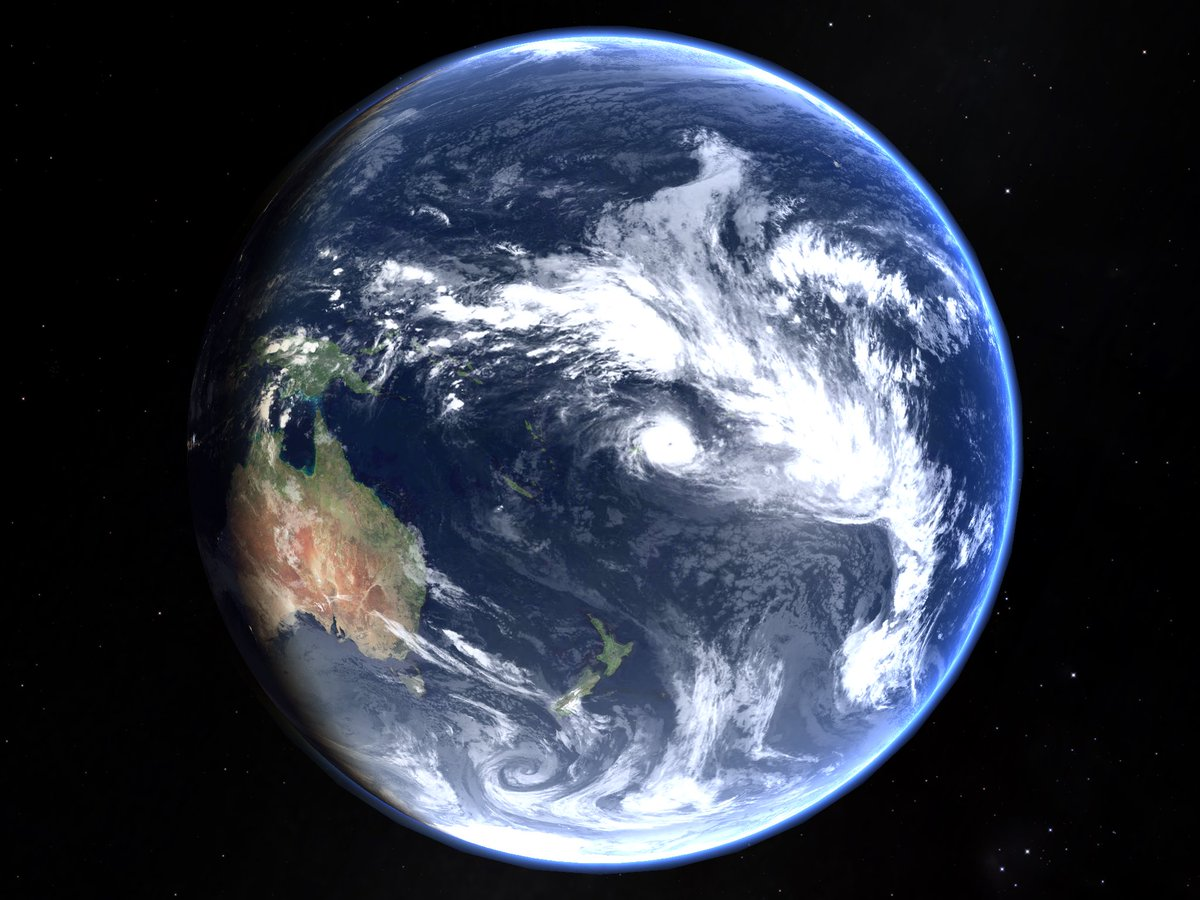
\includegraphics[width=1.0\hsize]{winston.jpg}
%  \begin{itemize}
%
% \item Geophysical Flows:
%
% atmospheres and oceans, rotation is important
% \end{itemize}
%    \end{columns}
%}
%
%%%%%%%%%%%%%%%%%%%%%%%%%%%%%%%%
%
%\frame{
%  \frametitle{Transformation into Rotating Reference Frame}
%  \begin{columns}
%  \column{0.5\textwidth}
%\hskip1cm \includegraphics[width=1.0\hsize]{rt_01.pdf}
%
%\column{0.5\textwidth}
%
%%\pause
%%Velocity in $R_{f}$: ${{\bf{u}}_{f}}$
%%\[{{\bf{u}}_{f}=\frac{d_{f}{\bf{x}}}{dt}}\]
%
%\end{columns}
%
%}
%
%
%
%\frame{
%  \frametitle{Transformation into Rotating Reference Frame}
%  \begin{columns}
%  \column{0.5\textwidth}
%\hskip1cm \includegraphics[width=1.0\hsize]{rt_02.pdf}
%
%
%\column{0.5\textwidth}
%
%%Velocity in $R_{f}$: ${{\bf{u}}_{f}}$
%%\[{{\bf{u}}_{f}=\frac{d_{f}{\bf{x}}}{dt}}\]
%
%
%\end{columns}
%
%}
%
%
%
%
%\frame{
%  \frametitle{Transformation into Rotating Reference Frame}
%  \begin{columns}
%  \column{0.5\textwidth}
%\hskip1cm \includegraphics[width=1.0\hsize]{rt_03.pdf}
%
%
%\column{0.5\textwidth}
%
%%Velocity in $R_{f}$: ${{\bf{u}}_{f}}$
%%\[{{\bf{u}}_{f}=\frac{d_{f}{\bf{x}}}{dt}}\]
%
%
%\end{columns}
%
%}
%
%
%
%
%\frame{
%  \frametitle{Transformation into Rotating Reference Frame}
%  \begin{columns}
%  \column{0.5\textwidth}
%\hskip1cm \includegraphics[width=1.0\hsize]{rt_04.pdf}
%
%
%\column{0.5\textwidth}
%
%%Velocity in $R_{f}$: ${{\bf{u}}_{f}}$
%%\[{{\bf{u}}_{f}=\frac{d_{f}{\bf{x}}}{dt}}\]
%
%
%\end{columns}
%
%}
%
%
%
%
%\frame{
%  \frametitle{Transformation into Rotating Reference Frame}
%  \begin{columns}
%  \column{0.5\textwidth}
%\hskip1cm \includegraphics[width=1.0\hsize]{rt_05.pdf}
%
%\column{0.5\textwidth}
%
%\pause
%Velocity in $R_{f}$: ${{\bf{u}}_{f}}$
%\[{{\bf{u}}_{f}=\frac{d_{f}{\bf{x}}}{dt}}\]
%
%%\pause
%Velocity in $R_{r}$: ${{\bf{u}}_{r}}$
%\[{{\bf{u}}_{r}=\frac{d_{r}{\bf{x}}}{dt}}\]
%
%\pause
%For some vector ${\bf{x}}$,
%\[{\frac{d_{f}{\bf{x}}}{dt}=\frac{d_{r}{\bf{x}}}{dt}+{\Omega\times{\bf{x}}}}\]
%
%%\pause{Take the vector ${\bf{u}}_{f}$,}
%%{\[{\frac{d_{f}{\bf{u}}_{f}}{dt} = \frac{d_{r}{\bf{u}}_{f}}{dt}+{\Omega\times{\bf{u}}_{f}}}\]}
%
%
%\end{columns}
%
%}
%
%
%
%\frame{
%  \frametitle{Transformation into Rotating Reference Frame}
%  \begin{columns}
%  \column{0.45\textwidth}
%\hskip1cm \includegraphics[width=0.75\hsize]{rt_05.pdf}\\
%
%In $R_{f}$: $\qquad{{\bf{u}}_{f}=\frac{d_{f}{\bf{x}}}{dt}}$
%
%
%In $R_{r}$: $\qquad{{\bf{u}}_{r}=\frac{d_{r}{\bf{x}}}{dt}}$
%
%
%For vector ${\bf{x}}$,
%
%$\qquad\qquad{\frac{d_{f}{\bf{x}}}{dt}=\frac{d_{r}{\bf{x}}}{dt}+{\Omega\times{\bf{x}}}}$
%
%\column{0.6\textwidth}
%\pause
%{Take the vector ${\bf{u}}_{f}$,}
%{\[{\frac{d_{f}{\bf{u}}_{f}}{dt} = \frac{d_{r}{\bf{u}}_{f}}{dt}+{\Omega\times{\bf{u}}_{f}}}\]}
%\pause{\[= \frac{d_{r}}{dt}\left[\frac{d_{r}{\bf{x}}}{dt}+{\Omega\times{\bf{x}}}\right] +{\Omega\times{\left[\frac{d_{r}{\bf{x}}}{dt}+{\Omega\times{\bf{x}}}\right]}}\]}
%\pause{\[= \frac{d_{r}}{dt}\left[{\bf{u}}_{r}+{\Omega\times{\bf{x}}}\right] +{\Omega\times{\left[{\bf{u}}_{r}+{\Omega\times{\bf{x}}}\right]}}\]}
%\pause{\[= \frac{d_{r}{\bf{u}}_{r}}{dt}+\frac{d_{r}}{dt}\left[{\Omega\times{\bf{x}}}\right] +{\Omega\times{\bf{u}}_{r}+{\Omega\times\Omega\times{\bf{x}}}}\]}
%\pause{\[{\frac{d_{f}{\bf{u}}_{f}}{dt}} = \frac{d_{r}{\bf{u}}_{r}}{dt}+2{\Omega\times{\bf{u}}_{r}+{\Omega\times\Omega\times{\bf{x}}}}\]}
%\end{columns}
%
%}
%

%
%\frame{
%  \frametitle{Transformation into Rotating Reference Frame}
%
%\[{\frac{d_{f}{\bf{u}}_{f}}{dt}} \quad =\quad \frac{d_{r}{\bf{u}}_{r}}{dt}\quad+\quad2{\Omega\times{\bf{u}}_{r}\quad+\quad{\Omega\times\Omega\times{\bf{x}}}}\]
%\pause
%$\quad\qquad$accel. in $R_{f}$ \pause = accel. in $R_{r}$  \pause + $\quad$  Coriolis \pause $\quad$ + $\quad$ centripetal
%
%\hskip1cm
%
%\pause
%
%Substitute back into momentum equation for fixed frame of reference:
%
%  \[\frac{D_{f}{\bf{u}}_{f}}{Dt} =  {\bf{g}} - \frac{\nabla{p}}{\rho} + \nu \nabla^2{\bf{u}}_{f}\]
%
%\pause
%
% % \begin{alertblock}
%\[ \frac{D_{r}{\bf{u}}_{r}}{Dt} + 2{\Omega\times{\bf{u}}_{r}}  + {\Omega\times\Omega\times{\bf{x}}}=  {\bf{g}} - \frac{\nabla{p}}{\rho} + \nu \nabla^2{\bf{u}}_{r}\]
%%  \end{alertblock}
%
%
%}
%%%%%%%%%%%%%%%%%%%%%%%%%%%%%%%%%%%%%%%%%%%%%%%%%%%%%%%%%%%%%%%%%%%%%%%%%%%%%%%%%%%%%%%%%%%%%

\frame{
  \frametitle{Transform from Inertial to Rotating Reference Frame}

\[{\frac{d_{f}{\bf{u}}_{f}}{dt}} \quad =\quad \frac{d_{r}{\bf{u}}_{r}}{dt}\quad+\quad2{\Omega\times{\bf{u}}_{r}\quad+\quad{\Omega\times\Omega\times{\bf{x}}}}\]

$\quad\qquad$accel. in $R_{f}$ = accel. in $R_{r}$  + $\quad$  Coriolis $\quad$ + $\quad$ centripetal

\hskip1cm

Substitute back into momentum equation for fixed frame of reference:

\[\frac{D_{f}{\bf{u}}_{f}}{Dt} =  {\bf{g}} - \frac{\nabla{p}}{\rho} + \nu \nabla^2{\bf{u}}_{f}\]


\begin{alertblock}{}
 \[ \frac{D_{r}{\bf{u}}_{r}}{Dt} + 2{\Omega\times{\bf{u}}_{r}}  + {\Omega\times\Omega\times{\bf{x}}}=  {\bf{g}} - \frac{\nabla{p}}{\rho} + \nu \nabla^2{\bf{u}}_{r}\]
\end{alertblock}



}

\frame{
  \frametitle{Geopotential}


Focus on the term ${\Omega\times\Omega\times{\bf{x}}}$
\pause

Triple vector cross product:
\[{\bf{a}}\times{{\bf{b}}}\times{{\bf{c}}} = {\bf{b}}({\bf{a}}\cdot{{\bf{c}}})-{\bf{c}}({\bf{a}}\cdot{{\bf{b}}})\]
\pause
\[{\Omega\times\Omega\times{\bf{x}}} = {\Omega(\Omega\cdot{\bf{x}})}-{{\bf{x}}(\Omega\cdot\Omega)}\]
\pause
Substitute the along-axis (${\bf{z}}$) and off-axis (${\bf{r}}$) components for ${\bf{x}}$:

\[{{\Omega\times\Omega\times{\bf{x}}} = {\Omega(\Omega\cdot({\bf{r}}+{\bf{z}}))}-({\bf{r}}+{\bf{z}})(\Omega\cdot\Omega)}\]
\pause
\[{{\Omega\times\Omega\times{\bf{x}}} = -{\bf{r}}\Omega^{2}}\]
\pause
Make this quantity a potential in ${\bf{r}}$ by integrating with respect to ${\bf{r}}$:

\[{{\Omega\times\Omega\times{\bf{x}}} = -\nabla\frac{{\bf{r}}^{2}\Omega^{2}}{2}}\]

}



\frame{
  \frametitle{Geopotential}

\[{{\Omega\times\Omega\times{\bf{x}}} = -\nabla\frac{{\bf{r}}^{2}\Omega^{2}}{2}}\]
\pause
Incorporate it together with the gravity term:

\[{\bf{g^{*}}} = {\bf{g}}-{{\Omega\times\Omega\times{\bf{x}}} = {\bf{g}}+\nabla\frac{{\bf{r}}^{2}\Omega^{2}}{2}} = -{\nabla{\Phi}}\]
\pause
into a term called the geopotential  $\Phi = \Phi_{g} - \nabla\frac{{\bf{r}}^{2}\Omega^{2}}{2}$

\hskip1cm

\pause

Substitute back into the momentum equation to give,

 \[\frac{D_{r}{\bf{u}}_{r}}{Dt} + 2{\Omega\times{\bf{u}}_{r}} =  {\bf{g^{*}}} - \frac{\nabla{p}}{\rho} + \nu \nabla^2{\bf{u}}_{r}\]

}



%%%%%%%%%%%%%%%%%%%%%%%%%%%%%%%%%%%%%%%%%%%%%%%%%%%%%%%%%%%%%%%%%%%%%%%%%%%%%%%%%%%%%%%%%%%%%%
%
%
%
%\frame{
%  \frametitle{Coriolis Force: $2\Omega\times{{\bf{u}}}$}
%
%\includegraphics[height=0.90\vsize]{coriolis_01.pdf}\\
%
%}
%
%
%
%\frame{
%  \frametitle{Coriolis Force: $2\Omega\times{{\bf{u}}}$}
%
%\includegraphics[height=0.90\vsize]{coriolis_02.pdf}\\
%
%}
%
%
%\frame{
%  \frametitle{Coriolis Force: $2\Omega\times{{\bf{u}}}$}
%
%\includegraphics[height=0.90\vsize]{coriolis_03.pdf}\\
%
%}
%
%
%\frame{
%  \frametitle{Coriolis Force: $2\Omega\times{{\bf{u}}}$}
%
%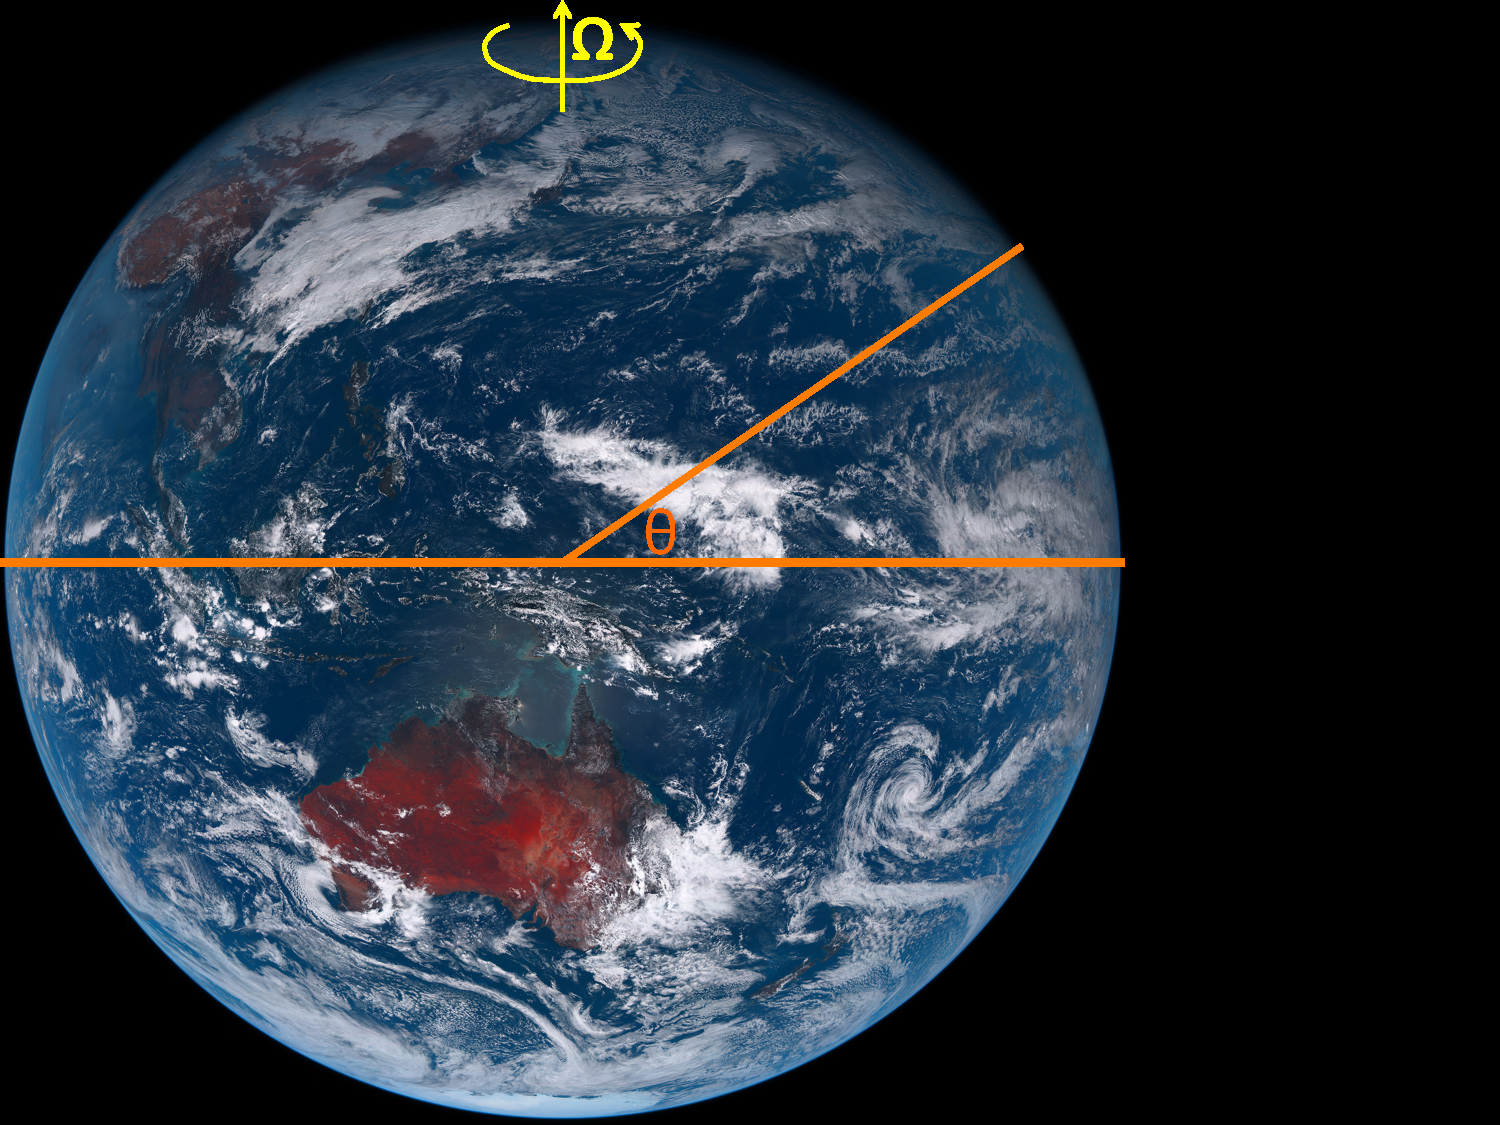
\includegraphics[height=0.90\vsize]{coriolis_04.pdf}\\
%
%}
%
%
%\frame{
%  \frametitle{Coriolis Force: $2\Omega\times{{\bf{u}}}$}
%
%\includegraphics[height=0.90\vsize]{coriolis_05.pdf}\\
%
%}
%
%
%\frame{
%  \frametitle{Coriolis Force: $2\Omega\times{{\bf{u}}}$}
%
%\includegraphics[height=0.90\vsize]{coriolis_06.pdf}\\
%
%}
%
%
%\frame{
%  \frametitle{Coriolis Force: $2\Omega\times{{\bf{u}}}$}
%
%\includegraphics[height=0.90\vsize]{coriolis_07.pdf}\\
%
%}
%
%
%\frame{
%  \frametitle{Coriolis Force: $2\Omega\times{{\bf{u}}}$}
%
%\includegraphics[height=0.90\vsize]{coriolis_08.pdf}\\
%
%}
%
%
%\frame{
%  \frametitle{Coriolis Force: $2\Omega\times{{\bf{u}}}$}
%
%\includegraphics[height=0.90\vsize]{coriolis_09.pdf}\\
%
%}
%
%
%\frame{
%  \frametitle{Coriolis Force: $2\Omega\times{{\bf{u}}}$}
%
%\includegraphics[height=0.90\vsize]{coriolis_10.pdf}\\
%
%}
%
%
%\frame{
%  \frametitle{Coriolis Force: $2\Omega\times{{\bf{u}}}$}
%
%\includegraphics[height=0.90\vsize]{coriolis_11.pdf}\\
%
%}
%
%
%\frame{
%  \frametitle{Coriolis Force: $2\Omega\times{{\bf{u}}}$}
%
%\includegraphics[height=0.90\vsize]{coriolis_12.pdf}\\
%
%}
%
%
%\frame{
%  \frametitle{Coriolis Force: $2\Omega\times{{\bf{u}}}$}
%
%\includegraphics[height=0.90\vsize]{coriolis_13.pdf}\\
%
%}
%
%
%\frame{
%  \frametitle{Momentum Equation on a Rotating Planet}
%
%  \begin{exampleblock}<1->{Momentum Equation in Rotating Frame}
%       \[\sd{\vc{u}}{t} + 2\pmb{\Omega}\times\vc{u} =  \vc{g} - \frac{\nabla p}{\rho} + \nu \nabla^2 \vc{u}\]
%\end{exampleblock}
%
%}
%
%
%
%\frame{
%  \frametitle{Question: Geopotential Surface}
%  \begin{columns}
%  \column{0.6\textwidth}
%    \includegraphics[width=1.0\hsize]{geopotential1.pdf} 
%
%   \column{0.3\textwidth}
%   \[\vc{g^*} = \vc{g} + \pmb{\nabla}(\frac{1}{2}\pmb{\Omega}^2{r}^2)\]
%%   \[\vc{z^*} = \vc{z} + \frac{{\Omega}^2{r_{e}}^2\textrm{cos}^{2}{\Theta}}{2g}\]
%
%What is the difference in distance between the centre of Earth and the geopotential surface at the pole and equator?
%
%   \[{\Omega=7.3\times{10^{-5}}\textrm{s}^{-1}}\]
%   \[{r_{e}}=6.37\times{10^{6}}\textrm{m}\]
%   \[{\bf{g}}=9.81ms^{-2}\]
%%   ${z^*}$ at pole is $\sim$11km closer to the centre of the Earth than equator
%   
%  \end{columns}
% 
%}
%
%%%%%%%%%%%%%%%%%%%%%%%%%%%%%%%%%%%%%%%%%%%%%%%%%%%%%%%%%%%%%%%%%%%%%%%%%%%%%%%%%%%%%%%%%%%%%
%

%\frame{
%  \frametitle{Atmosphere: Hurricane Katrina \& Cyclone Pam}
% \begin{columns}
% \column{0.5\textwidth}
%  \includegraphics[width=0.9\hsize]{katrina_in_gulf650.jpg}\\
%  
%  \column{0.5\textwidth}
%  \includegraphics[width=0.9\hsize]{cyclone_pam.jpg}\\
%  
%\end{columns}
%
%}

%\frame{
%  \frametitle{Ocean: Gulf Stream \& East Australian Current (SST)}
%  
% \begin{columns}
% \column{0.5\textwidth}
% \includegraphics[width=0.9\hsize]{gulf_stream.jpeg}\\
% 
% \column{0.5\textwidth}
% \includegraphics[width=0.9\hsize]{east_australian_current_fig1.jpg}\\
% 
%\end{columns}
%
%}

%\frame{
%  \frametitle{Circulation of Earth's outer core}
% 
% The outer core  (almost entirely liquid iron) generates the Earth's magnetic field.
% 
% \begin{center}
% \includegraphics[width=0.8\hsize]{geomag.jpg}
%\end{center}
%
%}


%\section{Transformation to a Rotating Reference Frame}
%\frame{
%  \frametitle{Transformation to Rotating Reference Frame}
%
%  \begin{columns}
%  \column{0.55\textwidth}
%\begin{alertblock}{Assumption in N-S equation}
%\begin{itemize}
%  \item \textbf{Inertial} reference frame
%  \item It implies \textbf{ motions timescale $<<$ rotation period} of the planet.
%  \item Hence, N-S $\Rightarrow$ rapid or short lenghtscale motions.
%  \item \textbf{Slow or large-scale} motions: non-inertial terms (planetary rotation) must be considered.
%
%\end{itemize}
%\end{alertblock}
%  \column{0.45\textwidth}
%
%\hskip0.5cm \includegraphics[width=0.9\hsize]{PIA04866.jpg}
%\end{columns}
%\pause
%\begin{itemize}
%  \item Description of motions in a rotating frame.
%  \end{itemize}
%}

%\frame{
%  \frametitle{Transformation to Rotating Reference Frame}
%  \begin{columns}
%  \column{0.5\textwidth}
%
%\hskip1cm \includegraphics[width=0.45\hsize]{rotatingframe.pdf}
%
%Two frames:
%One fixed frame ($R_f$) and one frame ($R_r$) rotating at a speed $\Omega$. 
%
%Consider a point P at position $\vc{x}_r$, and velocity $\vc{u}_f$ in $R_f$ (resp. $\vc{u}_r$ in $R_r$).
%\hskip1.0cm
%For any vector $\vc{A}$, the relation $\nd{_f\vc{A}}{t} = \nd{_r\vc{A}}{t}+\pmb{\Omega}\times \vc{A}_r$ holds.
%
% \column{0.5\textwidth}
%\pause
%\hskip1.0cm
%
%Hence, $\vc{u}_f$ expresses as:
%\[\vc{u}_f = \nd{_f\vc{x}_r}{t} = \nd{_r\vc{x}_r}{t} + \pmb{\Omega} \times \vc{x}_r\]
%Consequently:
%\[\nd{_f\vc{u}_f}{t} = \nd{_r\vc{u}_f}{t} + \pmb{\Omega} \times \vc{u}_f\]
%\pause
%\[ = \nd{_r}{t}[ \nd{_r\vc{x}_r}{t} + \pmb{\Omega} \times \vc{x}_r] + \pmb{\Omega} \times [\nd{_r\vc{x}_r}{t} + \pmb{\Omega} \times \vc{x}_r]\]
%%\[ = \ns{_r\vc{x}_r}{t} + 2\pmb{\Omega}\times\nd{_r\vc{x}_r}{t} + \pmb{\Omega} \times \pmb{\Omega} \times \vc{x}_r\]
%\[ = \nd{_r\vc{u}_r}{t} + 2\pmb{\Omega}\times\vc{u}_r + \pmb{\Omega} \times \pmb{\Omega} \times \vc{x}_r\]
%
%%\pause
%{\color{blue} \textbf{\textit{accel in fixed fr} $ =$ \textit{accel in rot fr + Coriolis accel + centripetal accel}}}
%
%% \column{0.5\textwidth}
%%\pause
%%This relation holds for any vector quantity. Hence velocity in the fixed frame satisfies
%%\[\nd{_f\vc{u}_f}{t} = \nd{_r\vc{u}_f}{t} + \pmb{\Omega} \times \vc{u}_f\]
%%\pause
%%\[ = \nd{_r}{t}[ \nd{_r\vc{x}_r}{t} + \pmb{\Omega} \times \vc{x}_r] + \pmb{\Omega} \times [\nd{_r\vc{x}_r}{t} + \pmb{\Omega} \times \vc{x}_r]\]
%%\[ = \ns{_r\vc{x}_r}{t} + 2\pmb{\Omega}\times\nd{_r\vc{x}_r}{t} + \pmb{\Omega} \times \pmb{\Omega} \times \vc{x}_r\]
%%\[ = \nd{_r\vc{u}_r}{t} + 2\pmb{\Omega}\times\vc{u}_r + \pmb{\Omega} \times \pmb{\Omega} \times \vc{x}_r\]
%%\pause
%%{\color{blue} \textbf{\textit{accel in fixed fr} $ =$ \textit{accel in rot fr + Coriolis accel + centripetal accel}}}
%
%\end{columns}
%
%}
%
%\frame{
%  \frametitle{Transformation to Rotating Reference Frame}
%  
%Thus N-S momentum equation in a fixed frame
%  \[\sd{_f\vc{u}_f}{t} =  \vc{g} - \frac{\nabla p}{\rho} + \nu \nabla^2 \vc{u}_f\]
%becomes (on substituting the transformation to rotating frame): 
%  \[\sd{_r\vc{u}_r}{t} + 2\pmb{\Omega}\times\vc{u}_r =  \vc{g} - \pmb{\Omega} \times \pmb{\Omega}\times \vc{x}_r - \frac{\nabla p}{\rho} + \nu \nabla^2 \vc{u}_r\]
%  \pause
%  Centrifugal acceleration: correction to gravity acceleration $\vc{g}$:
%  \[\vc{g^*} = \vc{g} - \pmb{\Omega} \times \pmb{\Omega}\times \vc{x}_r = \vc{g} + \pmb{\nabla}(\frac{1}{2}\pmb{\Omega}^2r^2) = -\pmb{\nabla}\Phi\]
%   where $\Phi = \Phi_g - \frac{1}{2}\Omega^2r^2$ is the {\color{red} geopotential} ($\Phi_g$ the gravitational potential, $r$ the radius normal to the rotation axis). 
%   \pause 
%\begin{exampleblock}<3->{Momentum Equation in Rotating Frame}
% \[\sd{\vc{u}_r}{t} + \color{red}2\pmb{\Omega}\times\vc{u}_r\color{black} = \color{red} \vc{g^*} \color{black} - \frac{\nabla p}{\rho} + \nu \nabla^2 \vc{u}_r\]
%\end{exampleblock}
%
%}
%
%\section{Transformation to a Rotating Planet}
%\frame{
%  \frametitle{Geopotential Surface}
%  \begin{columns}
%  \column{0.6\textwidth}
%    \includegraphics[width=1.0\hsize]{geopotential1.pdf} 
%
%   \column{0.3\textwidth}
%   \[\vc{g^*} = \vc{g} + \pmb{\nabla}(\frac{1}{2}\pmb{\Omega}^2{r}^2)\]
%   \[\vc{z^*} = \vc{z} + \frac{{\Omega}^2{r_{e}}^2\textrm{cos}^{2}{\Theta}}{2g}\]
%   \[{\Omega=7.3\times{10^{-5}}\textrm{s}^{-1}}\]
%   \[{r_{e}}=6.37\times{10^{6}}\textrm{m}\]
%   ${z^*}$ at pole is $\sim$11km closer to the centre of the Earth than equator
%   
%  \end{columns}
% 
%}
%
%\frame{
%  \frametitle{Coriolis Force}
% \begin{columns}
%\column{0.4\textwidth}  
%%  \includegraphics[width=0.20\hsize]{jupiter__1__speedyspacebike.jpg} 
%% \hskip0.5cm \includegraphics[width=0.2\hsize]{rotationcomponents.pdf}
%  \includegraphics[width=1.0\hsize]{latitude.pdf}\\
% The magnitude of the Coriolis force varies with \textbf{latitude}. \\  
%\column{0.4\textwidth}
%    Local coordinate frame on the Earth surface\\
%    ($x$ E-W, $y$ N-S, $z$ vertical)
%  \pause
%\[\pmb{\Omega} = (0, \Omega cos{\theta}, \Omega sin{\theta})\]
%\pause
%at north pole: $sin{\theta}=1$, $\Omega_z = |\pmb{\Omega}| \hskip0.5cm (= 7.3\times 10^{-5}$\,s$^{-1}$)
%
%at equator: $sin{\theta}=0$, $\Omega_z = 0$\\
%\pause
%
%-Compare $U\Omega$ with $g$;\\
%$U$ ocean$<$0.1m/s,\\
%$U$ atmos$<$10m/s\\
%$U\Omega<<g$\\
%-\bf{Vert. Coriolis negligible}
%\end{columns}
%}
%
%\frame{
%  \frametitle{Coriolis Force}
% \begin{columns}
%\column{0.4\textwidth}  
%%  \includegraphics[width=0.20\hsize]{jupiter__1__speedyspacebike.jpg} 
%% \hskip0.5cm \includegraphics[width=0.2\hsize]{rotationcomponents.pdf}
%  \includegraphics[width=1.0\hsize]{latitude.pdf}\\
% The magnitude of the Coriolis force varies with \textbf{latitude}. \\  
%\column{0.4\textwidth}
%    Local coordinate frame on the Earth surface\\
%    ($x$ E-W, $y$ N-S, $z$ vertical)
%  \pause
%\[\pmb{\Omega} = (0, \Omega cos{\theta}, \Omega sin{\theta})\]
%\pause
% \[\pmb{2\Omega}\times\vc{u} = (-2\pmb{\Omega}v\textrm{sin}{\Theta},\,2\pmb{\Omega}u\textrm{sin}{\Theta},\,0)\]
%\pause
%\[=f{\hat{\vc{z}}} \times \vc{u}\]\\
%where $f = 2\pmb{\Omega}$sin$\Theta$ is the {\bf{Coriolis Parameter}}.\\
%\pause
%Coriolis in $x$ influenced by $v$!!
%
%
%\end{columns}
%}
%
%
%
%\frame{
%  \frametitle{Momentum Equation on a Rotating Planet}
%  Dropping $^*$ and $_r$:
%  \begin{exampleblock}<1->{Momentum Equation in Rotating Frame}
%       \[\sd{\vc{u}}{t} + 2\pmb{\Omega}\times\vc{u} =  \vc{g} - \frac{\nabla p}{\rho} + \nu \nabla^2 \vc{u}\]
%\end{exampleblock}
%       \pause
%  \begin{itemize}
%  \item $\vc{u}$ is velocity relative to the {\color{red} rotating frame}
%  \pause
%    \item LHS `inertial' terms: Fluid particle acceleration and Coriolis acceleration $2\pmb{\Omega}\times \vc{u}$
%  \pause
%  \item Coriolis and centrifugal accelerations: real effects attributed to \textit{virtual} forces.
%  \pause
%  \item Use \textbf{`right hand rule'} 
%  
%  (eg. for $\pmb{\Omega}$ upward and $\vc{u}$ horizontal, $\pmb{\Omega}\times \vc{u}$ is to the left of $\vc{u}$.
%  
%  Then if $RHS = 0$, $\sd{\vc{u}}{t}=-2\pmb{\Omega}\times \vc{u}$ is to the RIGHT of $\vc{u}$.)
%  \end{itemize}
%  
%}
%
%
%
%
%
%
%\frame{
%  \frametitle{Coriolis Force by Latitude}
%  \begin{columns}
%  \column{0.95\textwidth}
%   \includegraphics[height=0.9\vsize]{coriolis.png}
%    \end{columns}
%}
%
%
%\section{Vertical Momentum, Scaling and the Hydrostatic Approximation}
%\frame{
%  \frametitle{Scaling the Vertical Momentum}
%Euler equation $\sd{\vc{u}}{t} + 2\pmb{\Omega}\times\vc{u} =  \vc{g} - \frac{\nabla p}{\rho}$
%\pause
%has vertical component
%  \[\pd{w}{t} + u \pd{w}{x} +  v \pd{w}{y} +  w \pd{w}{z} + 2\Omega_x v - 2\Omega_y u = - g - \frac{1}{\rho}\pd{p}{z}\]
%  \pause
%  \begin{alertblock}{assume vertical scale $H <<$ horizontal lengthscale $L$}
% horizontal velocity scale $U$, timescale $T=L/U$, $w\sim UH/L$
%  \end{alertblock} 
%  \pause
%    Terms Magnitude:
%  \[ U^2H/L^2 + U^2H/L^2 + U^2H/L^2 +  U^2H/L^2 - \Omega_y U \sim -g -\Delta P/\rho H\]
%  \[H/L - \Omega L/U \sim -gL/U^2 - (\Delta P/\rho U^2)(L/H)\]
%  \pause
%Values: $\Omega\sim~ 10^{-4}$\,s$^{-1}$, $g\sim10$\,ms$^{-2}$, and assume $L\sim10^5-10^7$\,m; 
%
%Atmosphere $H\sim10^4$\,m, $U<10$\,ms$^{-1}$; Oceans $H\sim10^3$\,m, $U<1$\,ms$^{-1}$
%
%\pause
%Magnitude of terms: $H/L <0.1$, $\Omega L/U<10^{3}$, \textbf{$gL/U^2>10^{4}$} or \textbf{$10^6$}
%\pause
%  \begin{exampleblock}{LHS terms can be neglected $\rightarrow$ $\pd{p}{z}=-\rho g$ (\textbf{hydrostatic})}
%   \end{exampleblock}
%   
%}
%
%


%
%
%\frame{
%\frametitle{Next lecture}
%  \begin{itemize}
%  \item Horizontal momentum and the Coriolis force
%  \end{itemize}
%}

\end{document}

